\chapter{METODOLOGI}

% Ubah konten-konten berikut sesuai dengan isi dari metodologi

\section{Data dan Peralatan}

\textbf{Data}

Data yang digunakan dalam penelitian ini adalah data yang diperoleh dari Diabetic Retinopathy Analisis Grand challenge, berupa citra OCT \emph{angiography}

\begin{figure} [H] \centering
  % Nama dari file gambar yang diinputkan
  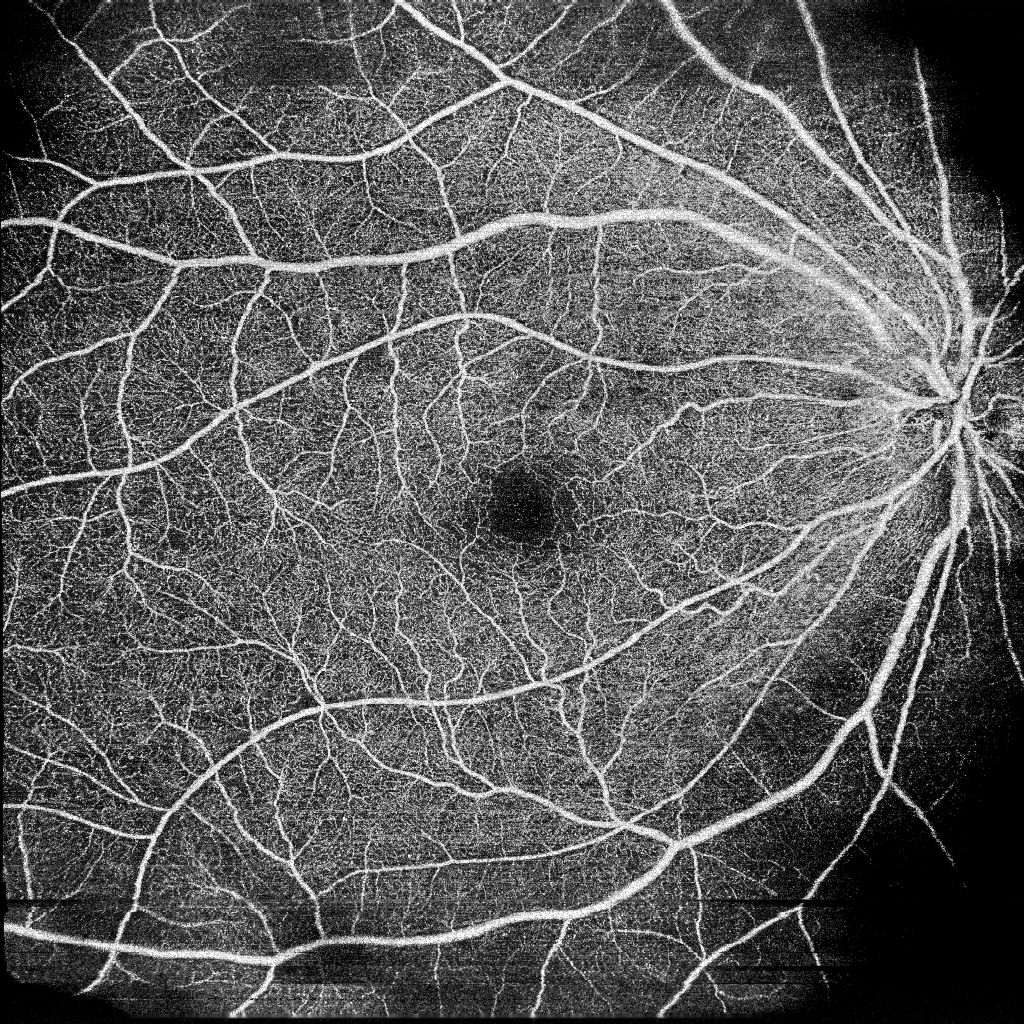
\includegraphics[scale=0.2]{gambar/exampleimage.png}
  % Keterangan gambar yang diinputkan
  \caption{Contoh Data Citra Retina}
  % Label referensi dari gambar yang diinputkan
  \label{fig:citraRetina}
\end{figure}

\textbf{Peralatan}

Dalam penelitian ini, penulis menggunakan komputer dengan sistem operasi Windows 11 dengan spesifikasi sebagai berikut:
\begin{itemize}
  \item Processor: Intel Core i5 12400F
  \item RAM: 16GB 3200MHz
  \item GPU: NVIDIA GeForce RTX 3060 Ti
  \subitem CUDA Cores: 4864
  \subitem Memory Config: 8 GB GDDR6
\end{itemize}

\emph{Software} yang digunakan dalam penelitian ini adalah sebagai berikut:
\begin{itemize}
  \item Jupyter Notebook
  \item Visual Studio Code
\end{itemize}

\section{Metode yang digunakan}

Perbandingan metode skenario yang digunakan dalam pelatihan model ResNet:
Dalam penelitian ini, dikarenakan oleh dataset yang sedikit dan ada class yang kurang representatif, dilakukan beberapa metode untuk penyeimbangan dataset.
\begin{itemize}
  \item Default
  
  Tidak ada Tindakan yang dilakukan untuk menyeimbangkan dataset. Metode ini dilakukan untuk variabel kontrol
  \item Penyesuaian \emph{Class-weight}
  
  Pada metode ini, dilakukan penambahan weight agar class yang underrepresented memiliki beban lebih tinggi
\end{itemize}


\begin{figure} [H] \centering
  % Nama dari file gambar yang diinputkan
  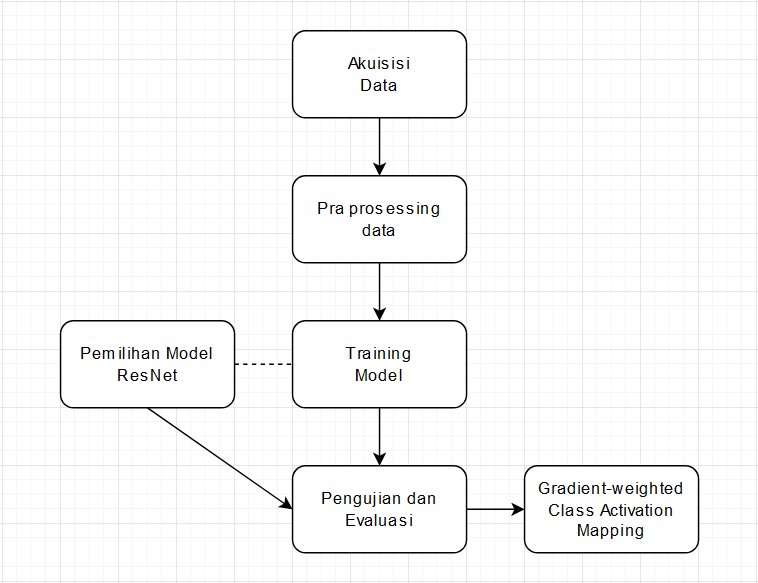
\includegraphics[scale=0.5]{gambar/diagramMethod.png}
  % Keterangan gambar yang diinputkan
  \caption{Diagram blok metodologi}
  % Label referensi dari gambar yang diinputkan
  \label{fig:diagramMethod}
\end{figure}

% Contoh penggunaan referensi dari gambar yang diinputkan
\subsection{Akuisisi Data}
Data yang digunakan dalam penelitian ini adalah data yang diperoleh dari Diabetic Retinopathy Analisis Grand challenge \parencite{drac_challenge_2023_10280359}. Data yang digunakan adalah data citra retina yang sudah diberi label berupa tingkat keparahan penyakit retinopati diabetik yang sebelumnya sudah melalui proses image assesment sehingga sudah siap digunakan untuk training model. Dataset ini berisikan 611 citra OCT-A yang telah diberi label. Dataset ini juga berisikan 386 citra OCT-A yang tidak berlabel untuk dijadikan testing dataset.

\subsection{Pra-pemrosesan Data}
Pra-pemrosesan data dilakukan untuk mempersiapkan data sebelum dilakukan proses pelatihan model. Pra-pemrosesan data yang dilakukan adalah konversi citra retina dari format .jpeg menjadi .png. Hal ini dilakukan karena format .png memiliki ukuran yang lebih kecil dibandingkan dengan format .jpeg. Selain itu, format .png juga tidak mengurangi kualitas citra retina. Pra-pemrosesan data juga dilakukan untuk membagi data menjadi data latih dan data uji. Data latih digunakan untuk melatih model sedangkan data uji digunakan untuk menguji model.

\subsection{ Model ResNet}
Model ResNet yang akan digunakan untuk dibandingkan dalam penelitian ini adalah model pre-trained resnet-18, resnet-34, resnet-50, resnet-101, dan resnet-152. Performa model-model tersebut akan dibandingkan dengan melihat nilai akurasi, \emph{loss}, dan \emph{val\_loss}.

\subsection{Pelatihan Model}
Pelatihan model dilakukan dengan menggunakan metode \emph{transfer learning}. Metode \emph{transfer learning} dilakukan dengan menggunakan model ResNet yang sudah dipilih dan sudah dilatih dengan dataset ImageNet.

\subsection{Pengujian dan Evaluasi}
Pengujian dan evaluasi dilakukan dengan menggunakan data uji. Pengujian dan evaluasi dilakukan dengan melihat nilai akurasi, \emph{loss}, dan \emph{val\_loss}. Selain itu, pengujian dan evaluasi juga dilakukan dengan melihat \emph{confusion matrix} dari model yang sudah dilatih, untuk dilihat nilai presisi, recall, dan F1 pada setiap kelasnya, untuk melihat performa model dalam memprediksi tingkat keparahan penyakit retinopati diabetik.

\subsection{Gradient-weighted Class Activation Mapping}
Grad-CAM digunakan untuk mengetahui faktor-faktor yang mempengaruhi model dalam memprediksi tingkat keparahan penyakit retinopati diabetik. Grad-CAM bekerja dengan menghitung gradien output model terhadap input, dan kemudian menggunakan gradien tersebut untuk memprediksi area input yang paling berkontribusi pada output model.
